\section{Problem definition}
With the advancements of technology,
people tried digitalizing every aspect of their life.
They renounced the traditional slow postal services in favour of
the modern fast email.
Digital photos gained popularity to the detriment of physical copies.
In the same way, CDs and other physical mediums were
forgotten with the arising of digital MP3s.


Over the past years, with the rise of the Internet,
even the idea of digitalizing one's life became old,
so people started to sync it with the cloud.
Hence, a new way of storing and transmitting data emerged: streaming.

\begin{figure}[h]
  \centering
  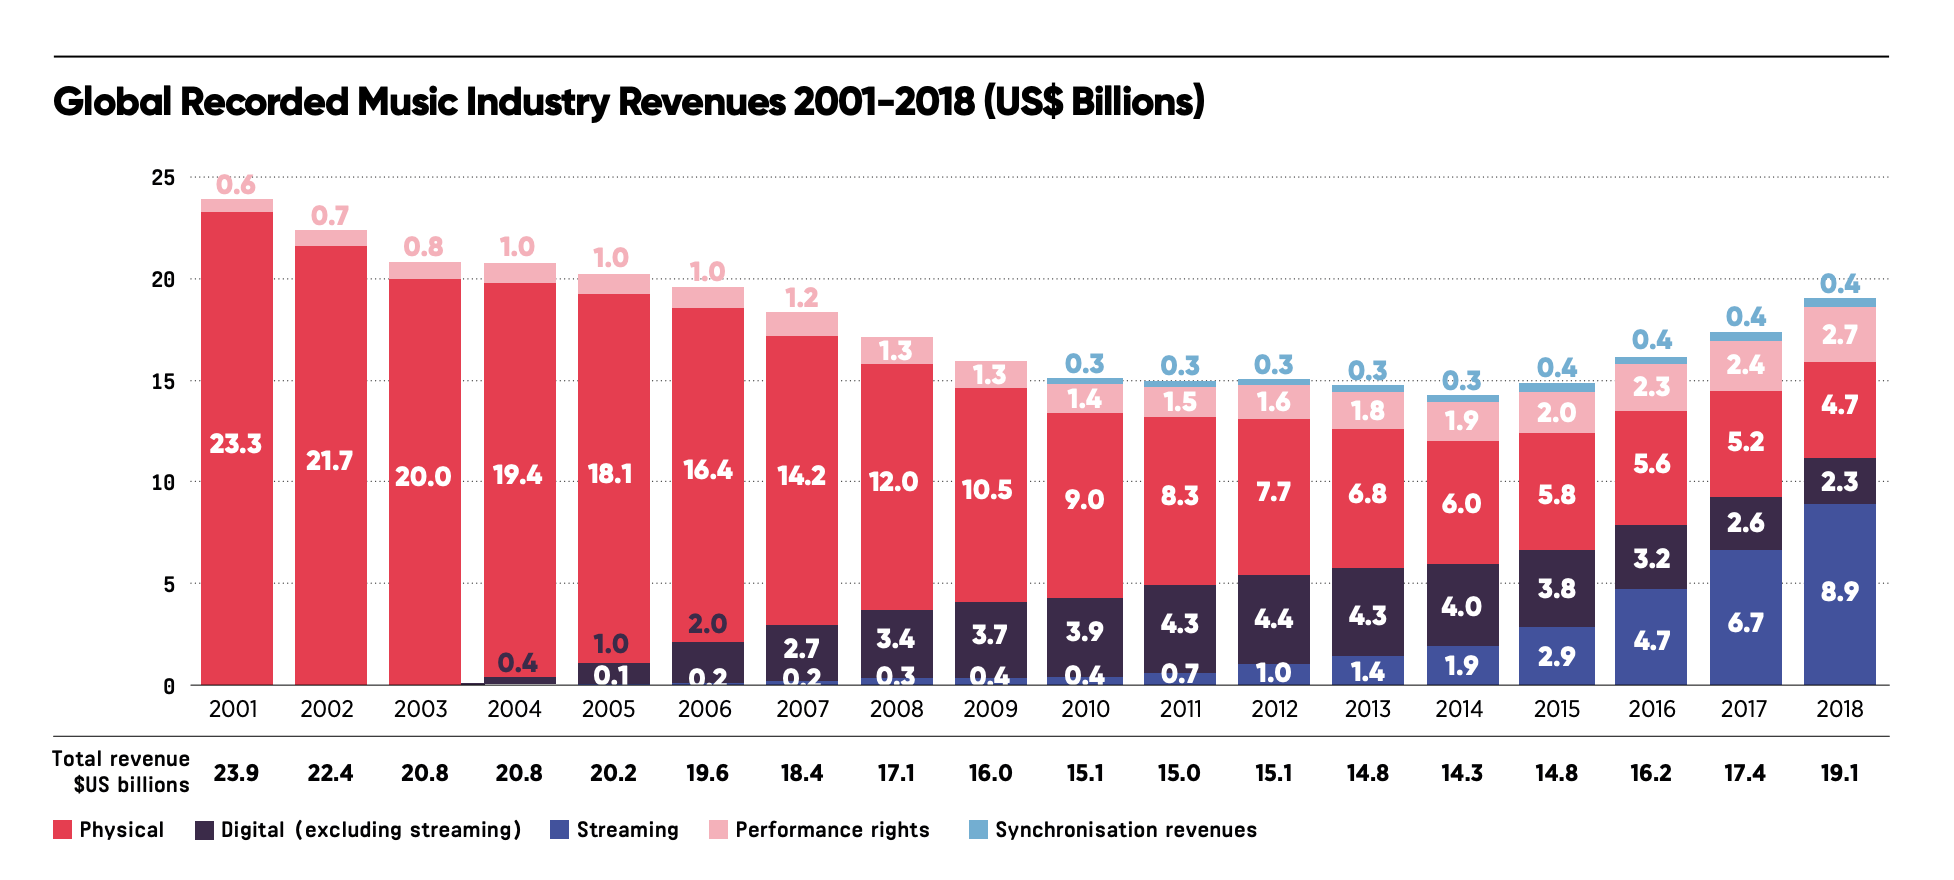
\includegraphics[width=1\textwidth]{ifpi}
  \caption{\emph{Global Recorded Music Industry Revenues 2001-2018  \cite{ifpi}}}
  \label{fig:ifpi}
\end{figure}

As shown in Figure\emph{~\ref{fig:ifpi}}, in the last decade,
the revenue of the music industry shifted,
going from physical to digital; nowadays,
the highest income is generated by streaming means.

With this change, one can easily compose and produce
music from their studio or even bedroom,
since it is not compulsory to be tied to a record label.
There are lots of successful independent musicians who
create music this way and the numbers are growing more
and more every year \cite{forbes}.

Even with all these developments,
the act of composing music did not drastically change in the last
few hundred years. If one wants to compose a song,
they should learn how to use instruments,
and how to put notes in such a manner that they sound good together.
Technology eased the process of composing,
but one must still learn chords, scales,
and other elements of music theory to make the process less hazardous.
Although music theory has a steep learning curve,
learning it helps express oneself musically.
Despite all these advancements,
there is a lack of tools facilitating the creative process.

This paper tries to fill the aforementioned deficit;
with the help of machine learning,
it proposes a system whose goal is to aid the aspiring musician easily
compose a song based on a given emotion.
It provides a way of generating new pieces of music without the need to master music theory.


\section{Orpheus's Sorrow's Approach}
\emph{Orpheus's Sorrow} is the name of the system mentioned before.
It is a client-server web application where a musician can input
emotion data and values to other parameters to visualize songs that this deep
neural network generated on the given data.
In the following sections,
it will be discussed the paper's approach related to music and emotion,
dataset creation, and the internal structure of the model.


\subsection{Music, emotions and machine learning}
% \begin{wrapfigure}{l}{0.4\textwidth}
%       \centering
%       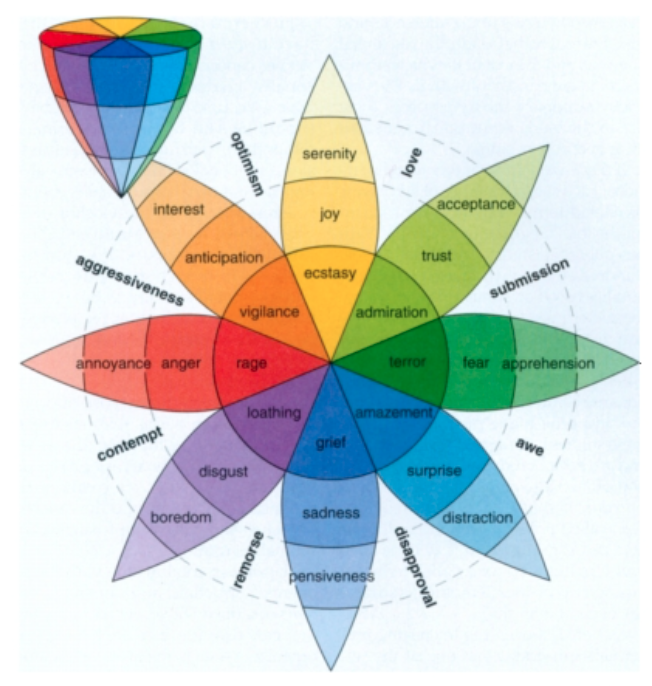
\includegraphics[width=0.35\textwidth]{plutchik}
%       \caption{\emph{Plutchik's wheel/cone of emotions \cite{plutchik}}}
%       \label{fig:plutchik}
% \end{wrapfigure}
\begin{figure}[h]
  \centering
  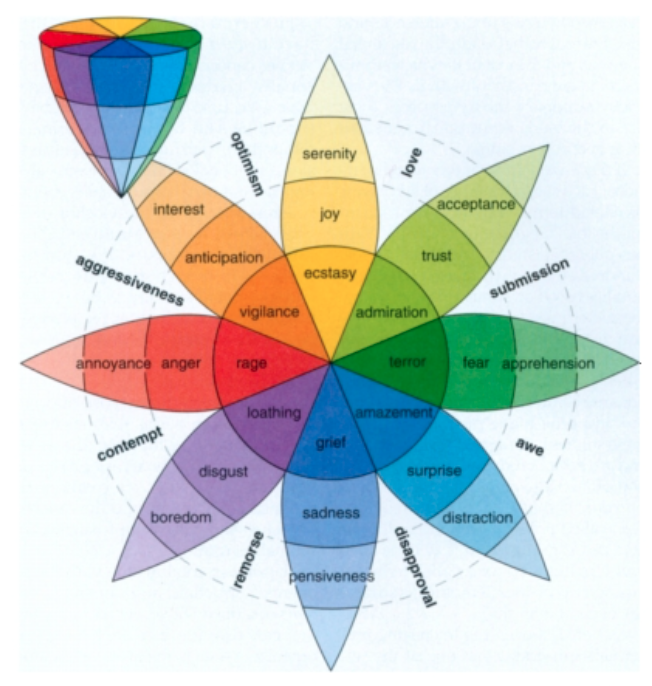
\includegraphics[width=0.5\textwidth]{plutchik}
  \caption{\emph{Plutchik's wheel/cone of emotions \cite{plutchik}}}
  \label{fig:plutchik}
\end{figure}
Music and emotion are highly connected,
one of the main goals of a composer being expressing his feelings through notes,
trying to reach his audience, and to induce them his mood and ideas.


When dealing with music classification based on the emotion it expresses,
there are multiple strategies for managing the sentiment data,
the most popular being tag-classification using some predefined emotions
or a regression approach representing the feeling through some variables.
Both of the approaches can be applied to the whole song or a subset of
features extracted manually or automatically.


The first one usually is paired with an existing model for emotions,
one of the most popular being Plutchik's wheel of emotions.
As can be seen in Figure\emph{~\ref{fig:plutchik}},
Plutchik circularly arranged the feelings,
proposing eight primary bipolar emotions:
surprise - anticipation, fear - anger, trust - disgust, joy - sadness.


\begin{wrapfigure}[10]{r}{0.5\textwidth}
  \centering
  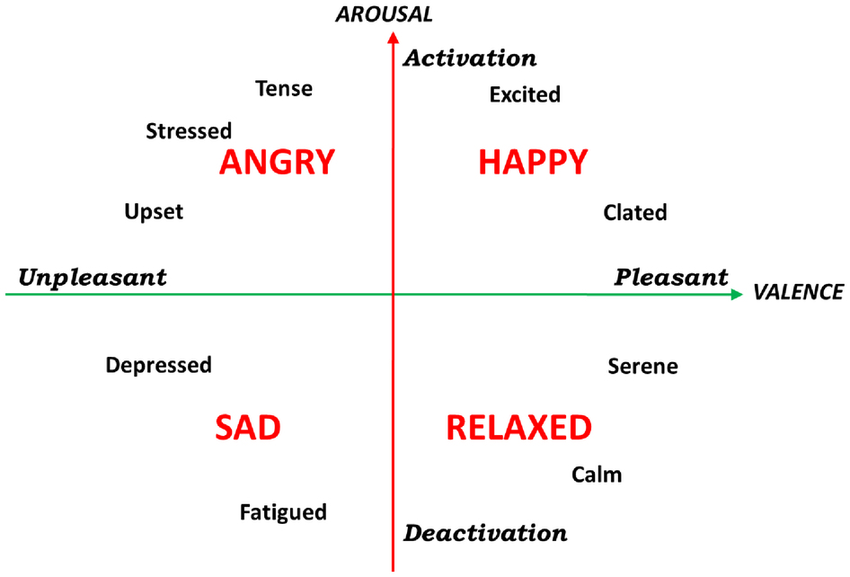
\includegraphics[width=0.45\textwidth]{thayers}
  \caption{\emph{Thayer's Model for Emotions (also named Russel's model) \cite{plutchik}}}
  \label{fig:thayers}
\end{wrapfigure}

When choosing the second, one frequently uses Thayers's
(also called Russell's) model. With this method,
every emotion can be described using two variables: valence and arousal.


As seen in Figure\emph{~\ref{fig:thayers}}, in this way,
feelings can be plotted on a cartesian system of coordinates obtaining
four general quadrants of emotions: happy, angry, sad, and relaxed.

\vspace{1cm}


\subsection{MIDIs and Emotion Dataset}


When discussing machine learning and neural networks,
one must know what data is available for their needs,
how to parse their data in a format they fully understand and maximizes
the potential of their data.


\begin{wrapfigure}[11]{L}{0.5\textwidth}
  \centering
  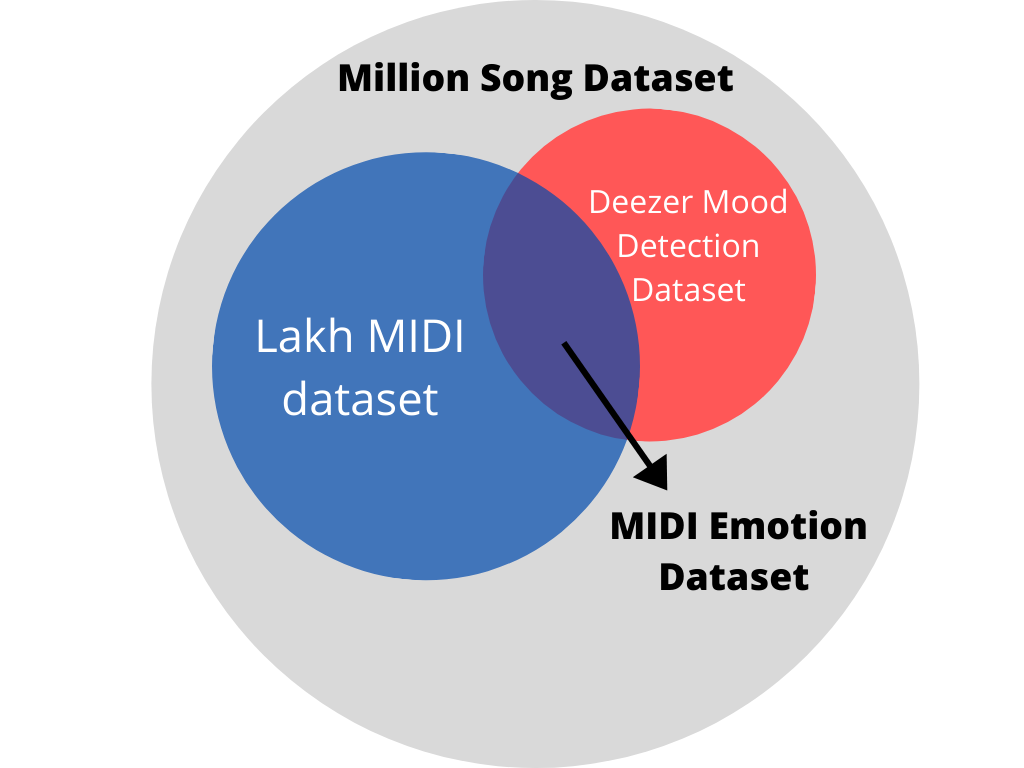
\includegraphics[width=0.45\textwidth]{dataset_creation}
  \caption{\emph{Merging existing datasets to create a new one}}
  \label{fig:dataset_creation}
\end{wrapfigure}
The model proposed uses MIDIs to store and handle the music information
data due to ease of manipulation, as mentioned before.
During quick research, there were not any free/public datasets
that satisfied the needs of the problem statement - a
dataset containing MIDIs with the emotion value (arousal and valence)
attached to each song. Hence there was a need to create a new dataset
by merging some of the existing ones to fulfill the requirements.
The merged datasets are the following:
\begin{itemize}
  \item{
        \textbf{Million Song Dataset} - a free compilation of metadata for a million contemporary common music records;\cite{themillion}
        }
  \item{
        \textbf{Lakh Midi Dataset} - set of over 150,000 unique MIDI files, over 40,000 being matched to entries in the dataset mentioned above;\cite{lakh}
        }
  \item{
        \textbf{Deezer Mood Detection Dataset} - valence and arousal dataset for over 10,000 songs also matched to the first-mentioned dataset.\cite{deezer}
        }
\end{itemize}



A visual representation of the sets is in Figure \emph{\ref{fig:dataset_creation}}.
It represents how the merging was performed.
The songs from the last two datasets were paired based on their
ID in the Million Song Dataset and then joined together with their relevant information.
The new dataset contains over 1800 MIDIs, with their respective valence and arousal,
enough data to train the model to see if this approach can have good results.

The obtained dataset was split into three parts: 80\% training data,
10\% validation data, 10\% testing data.
The training data was also augmented by shifting the pitch with several notes higher and lower.

\subsection{Model architecture}
Now, with the data ready to be fed to the model,
in the following paragraphs,
it will be discussed about its sampling and also about the structure of the model.

Feeding the MIDI file directly in the model
will not produce good results since there are too many irrelevant pieces of information
beyond our purpose, and that will confuse the network.
Before the actual training of the MIDI,
the files were transformed into piano rolls,
being sampled as a set of images.
A piano roll here consists of an image of type $noteRange * timing$.
The latter was chosen as 96, as used in \cite{hackerPoet},
mainly because almost all standard time signatures are dividing.
For the first one is chosen the same value since very few songs use the highest
and lowest pitches and also for symmetry's sake.

\begin{figure}[h]
  \centering
  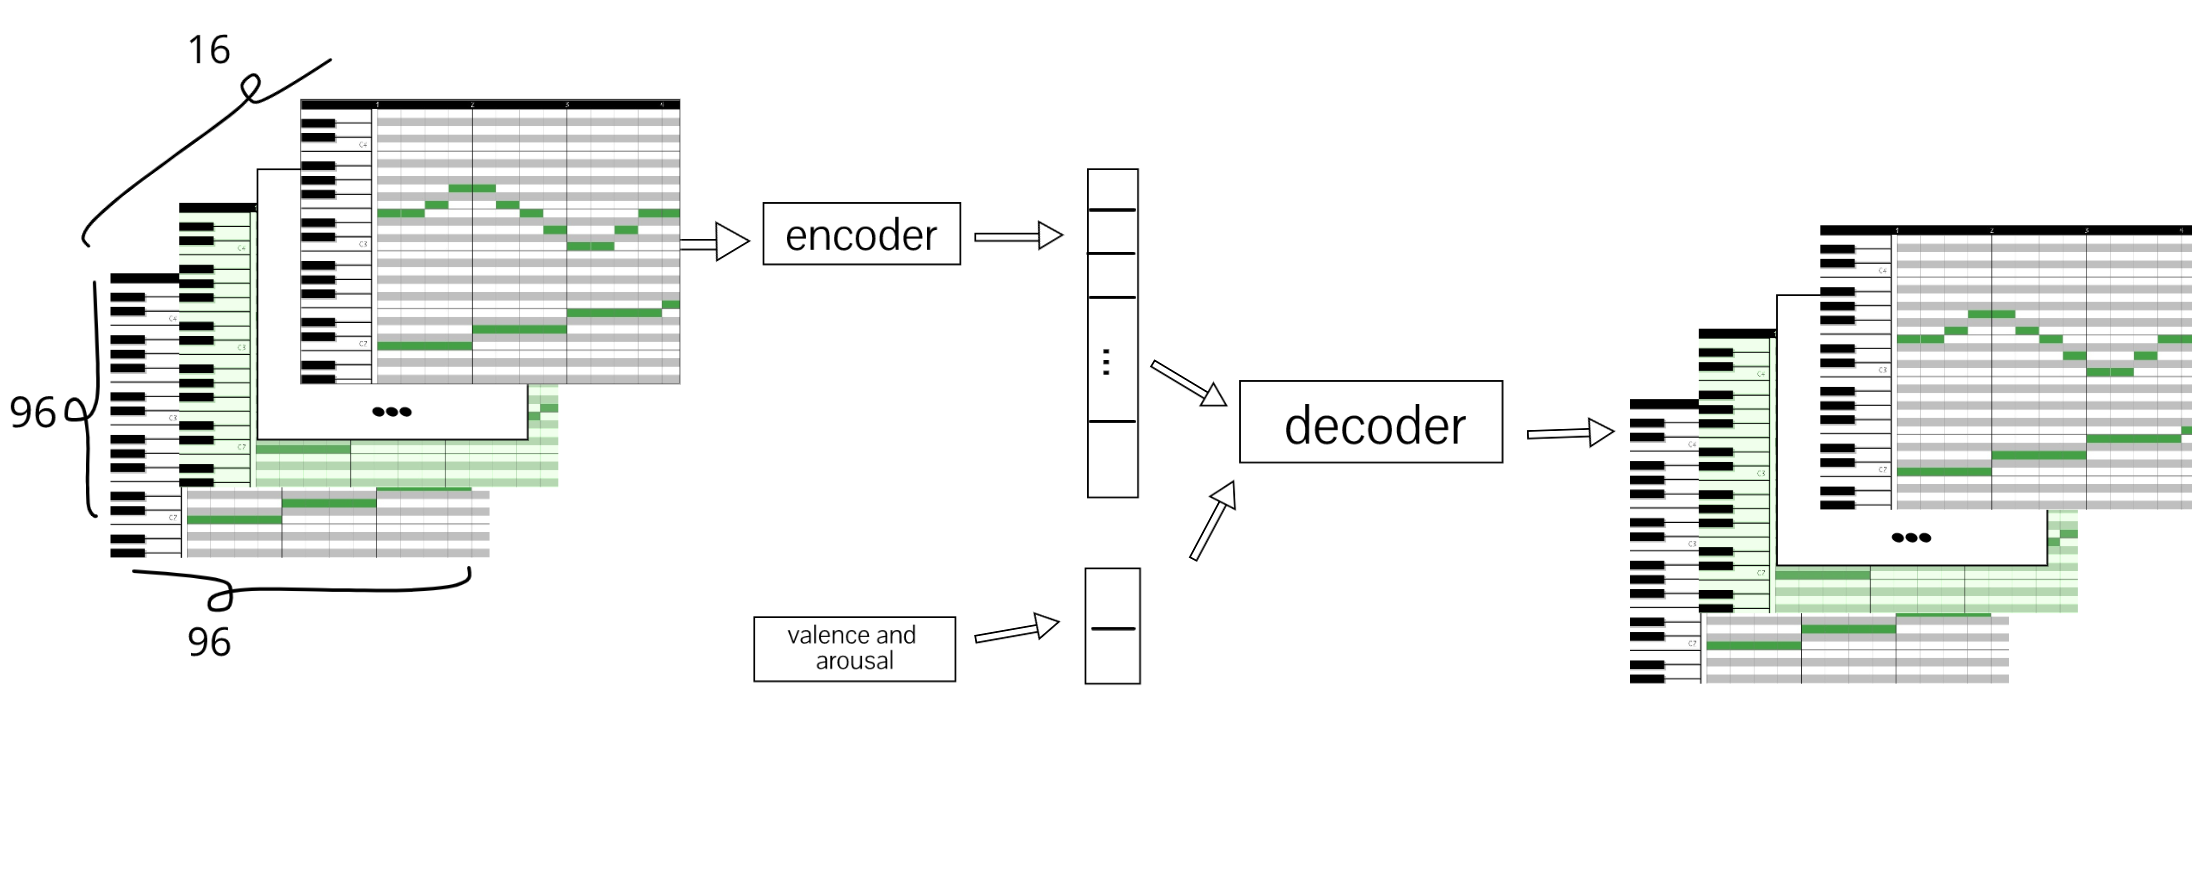
\includegraphics[width=1\textwidth]{model_short}
  \caption{\emph{Short description of paper's model}}
  \label{fig:model_short}
\end{figure}

As seen in Figure \emph{\ref{fig:model_short}},
the deep neural network consists of a deep autoencoder used to find the encoding of a song;
in other words, it finds the essential features of that piece of music.
It works similarly with the \cite{hackerPoet},
but the main highlight of this particular model is that to its encoding
are concatenated the valence and arousal values for each song,
this approach helping it to learn how to generate songs based on its input emotion data.


The composing works by creating an auxiliary model,
namely a Keras backend function,
that represents the decoder.
Its input is represented by two arrays,
the 48 values for the features the network identified,
and the emotional values; the set of piano rolls represents its output,
generating in this manner a new song.

Next, the main structure of the model will be presented,
with its primary layers and other parameters configured, as depicted in Figure \emph{\ref{fig:model}}.


For increasing its stability and speed, the model uses the batch-normalization layers.
Their purpose is to normalize the output of the prior activation layer
by subtracting the batch mean and dividing by its standard deviation,
reducing in this manner generalization errors, providing some regularization. \cite{batchNorm}

\begin{wrapfigure}[8]{l}{0.5\textwidth}
  \centering
  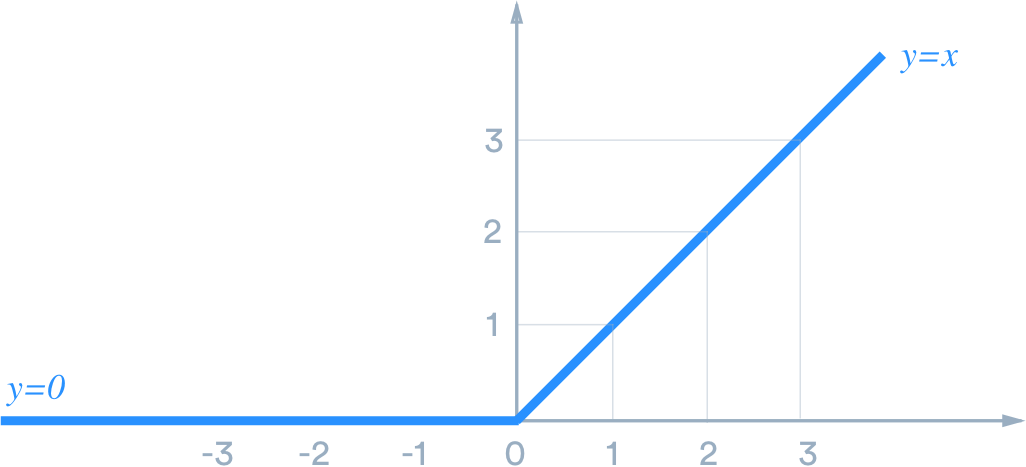
\includegraphics[width=0.3\textwidth]{relu}
  \caption{\emph{ReLU visual representation \cite{relu}}}
  \label{fig:relu}
\end{wrapfigure}

Another vital layer that helps to group the rolls in time-based sets is the time-distributed layer.
It is usually used as a middleware for 3D input; given a timestep,
it applies the same layer it wraps to each temporal slice of the same size as the timestep.\cite{keras}


\begin{figure}[hbt!]
  \centering
  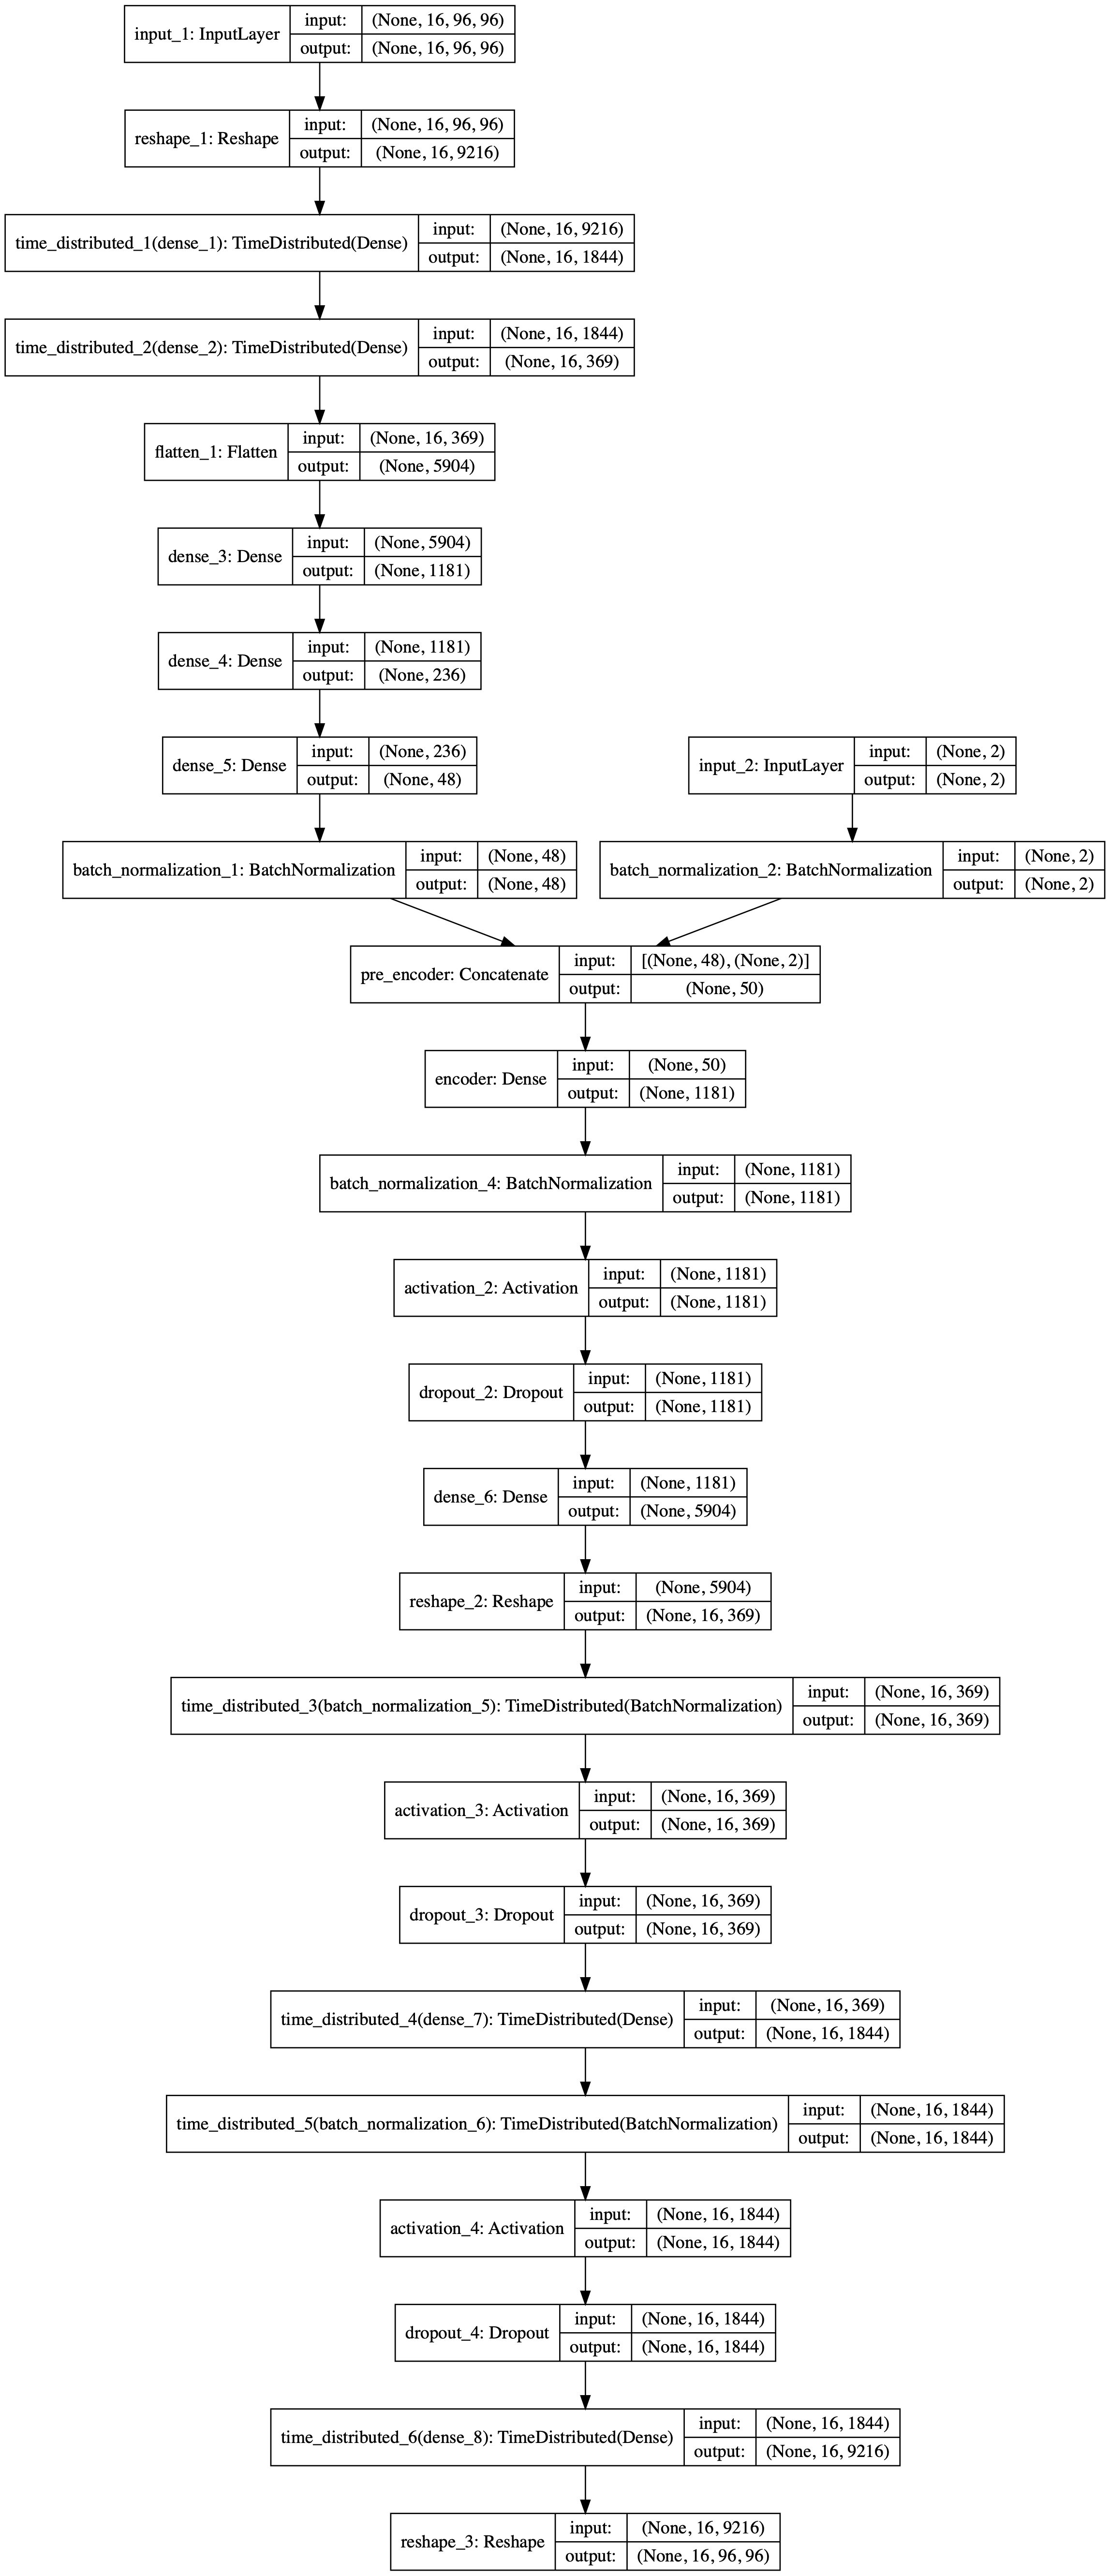
\includegraphics[height=0.8\paperheight, width=1\textwidth]{model}
  \caption{\emph{Structure of the model}}
  \label{fig:model}
\end{figure}

\clearpage

Another characteristic of our model is the activation function used -
ReLU(Rectified Linear Unit). Figure \emph{\ref{fig:relu}} represents the function mentioned before,
expressed mathematically as $y = max(0, x)$. It is not expensive to compute,
the model taking less time to train and run. \cite{relu}

The loss function used is the binary cross-entropy since the model
has to predict the probability of playing or not a note in its current context,
the mentioned function being the default used in binary classification problems.\cite{cross}


\subsection{Loss and Accuracy}


\begin{figure}[h]
  \centering
  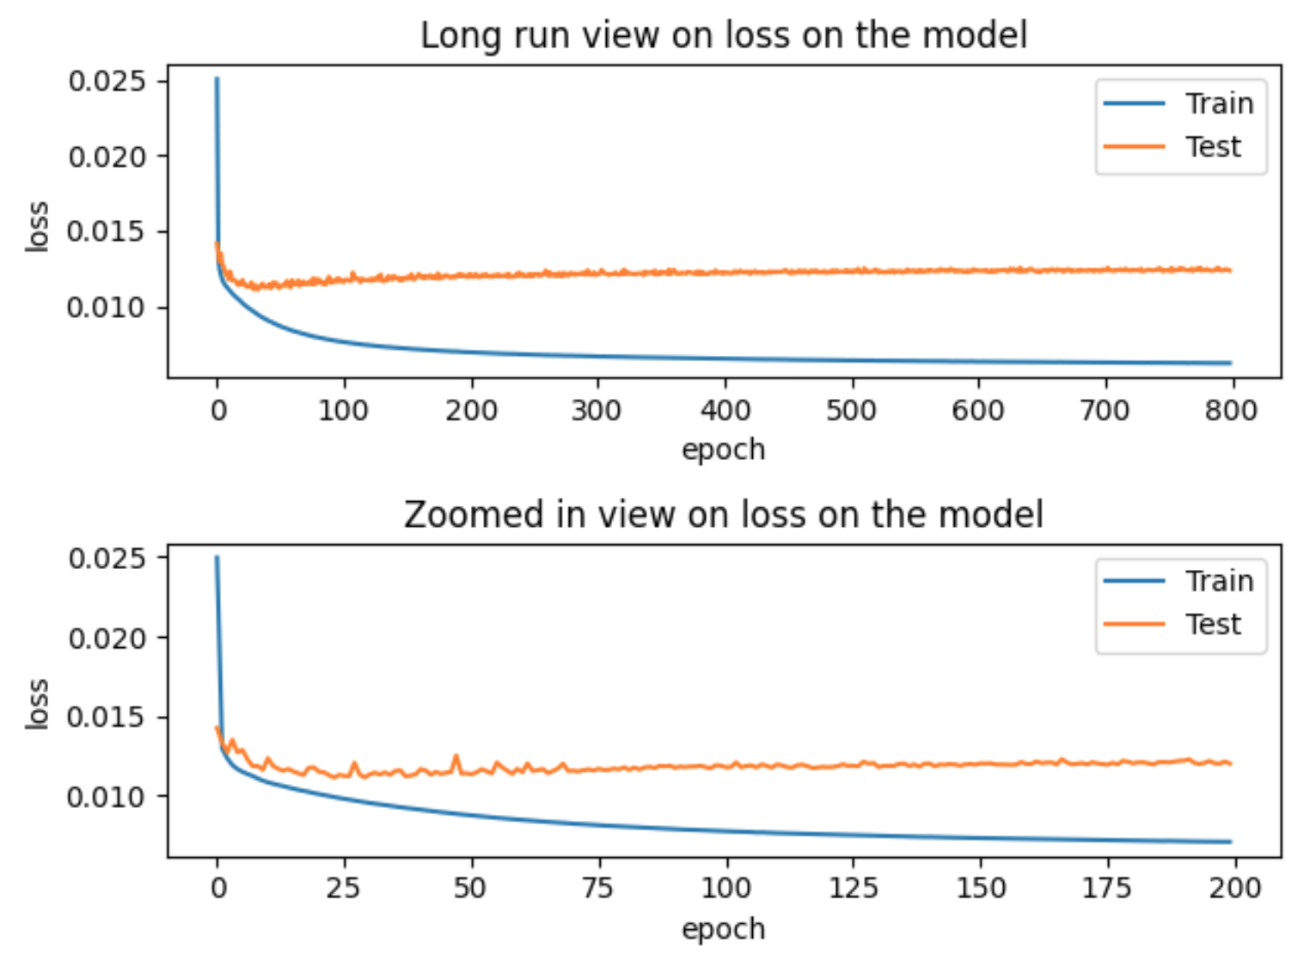
\includegraphics[width=.8\textwidth]{loss}
  \caption{figure}{\emph{Visual representation of loss}}
  \label{fig:loss}
\end{figure}

Researching other approaches for music composition influenced this paper,
even regarding the number of epochs one should train the model.
There are various empirical ways to estimate the most suitable number of epochs,
but since our dataset has not been used in other machine learning algorithms,
or since it does not have a large number of MIDIs, when training,
the model uses a callback that saves the model every n-th epoch.
In this manner, the training period cannot be ruined by overfitting
since the model can be reloaded at any saved moment.


From each model saved,
there can be retrieved some metadata about our songs.
This new information will be used when generating another song,
normalizing the given input through singular value decomposition,
reassuring that our features are in the normal range of our data.


As can be seen in Figure \emph{\ref{fig:loss}}, the top part, in the long run,
the model starts overfitting around the 200-300th epoch,
statement tested by the fact that every model above that period starts
composing the same songs regardless the input data. On the zoomed-in view,
the bottom part of the same Figure, the slope stats getting smaller around 175-200th epoch,
the model that was empirically chosen the best being the 190th epoch
due to its ability to compose the most exciting songs with a well-defined structure,
and other essential characteristics such as constant rhythm,
repeating structures (motifs). The accuracy curve, as seen in Figure \emph{\ref{fig:accuracy}},
starts flattening nearby the same interval for the train data and becomes
constant almost for the validation data.
When evaluating the chosen best model on the 10\% songs from the dataset
it was not trained with, the result obtained is 98\% accuracy.


\begin{figure}[h]
  \centering
  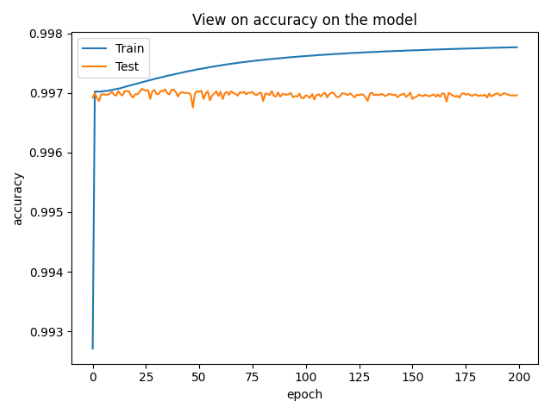
\includegraphics[width=.8\linewidth]{accuracy}
  \caption{\emph{Visual representation of accuracy}}
  \label{fig:accuracy}
\end{figure}



\section{Composing songs}
The discussed model, trained on the created dataset,
has excellent results regarding accuracy and loss,
but the generated songs do not get the same expected results regarding the emotion part.
Due to the smaller number of samples,
the learned features and also the valence and arousal values are very dependent,
meaning that given a composed song, at first listen,
the emotion denoted by the song is not clear, in the majority of cases.

Despite the vague emotion a composed song induces,
there are some characteristics that the model learned for each different quadrant
(see Figure \emph{\ref{fig:thayers}}).
For the first one (happy), most of the songs are using the major scale,
the most common characteristic of a happy song.
For the second one (angry), a preponderance of the songs is using minor scales,
part of them also tritones/dissonant chords,
the note density over time is much bigger,
the rhythm being galloping;
all of the above are features more frequently encountered in angry songs.
The fact that most of the MIDIs in the dataset from the last-mentioned quadrant
are metal or classical songs is also notable.
For the third quadrant (sad), a part of songs uses minor scales,
this being the quadrant with the most ambiguous results.
For the last quadrant (relaxed), some songs also use the major scale,
but the most notable fact is the low density of notes,
which is characteristic of slow-paced, calm songs.

